\documentclass[11pt]{article}
\usepackage[T1]{fontenc}
\usepackage{lmodern,microtype,amsmath,amssymb,amsthm,mathtools,xurl}
\usepackage[a4paper,margin=28mm]{geometry}
\usepackage{tikz}
\usetikzlibrary{arrows.meta,calc,patterns}
\usepackage[colorlinks=true,linkcolor=blue!55!black,citecolor=blue!55!black,urlcolor=blue!55!black]{hyperref}
\setlength{\emergencystretch}{2em}
\numberwithin{equation}{section}
\newtheorem{theorem}{Theorem}[section]
\newtheorem{lemma}[theorem]{Lemma}
\newtheorem{proposition}[theorem]{Proposition}
\newtheorem{corollary}[theorem]{Corollary}
\theoremstyle{remark}\newtheorem{remark}[theorem]{Remark}
\newcommand{\ii}{\mathrm i}
\newcommand{\dd}{\,\mathrm d}
\newcommand{\Log}{\operatorname{Log}}
\newcommand{\diag}{\operatorname{diag}}
\newcommand{\eps}{\varepsilon}
\title{Asymptotics of signed Newton coefficients near the quarter index}
\author{}\date{}
\begin{document}\maketitle

\begin{abstract}
A signed Newton coefficient in a root-of-unity tangle evaluation satisfies a second-order finite recurrence. At one quarter of the level its two characteristic roots have equal modulus but remain distinct. We prove a holomorphic asymptotic for the actual finite coefficient on a fixed neighborhood crossing that boundary. An analytic matrix reduction has exponentially small off-diagonal error on a domain chosen before the crossing width. The original high-index source supplies both initial channels. A strict cumulative action estimate suppresses its competing channel and every mode-conversion error, even for small complex color parameters. The selected product then admits exponentially accurate index interpolation, with the same nonzero amplitude, endpoint normalization and absolute shear action at both level parities. A local finite-window corollary retains the original affine lattice offsets. No estimate of the complementary global source or of a whole filling sum is asserted.
\end{abstract}

\section{The finite coefficient and the question}\label{qi:intro}

Rigorous asymptotics for finite-order recurrences form an established discrete WKB theory; see Costin and Costin \cite{CostinCostin} for a general treatment with smooth coefficients. We give the analytic matrix reduction used here directly, then identify the particular finite quantum source by its original endpoint. No novelty is claimed for the general diagonalization procedure.

Equal characteristic moduli do not by themselves determine an asymptotic of a finite recurrence. Below the equality point a locally smaller branch can become larger; an initially small component can then grow. We prove a local statement in which the actual source at a higher index, the cumulative relative actions and all conversions between the two branches are controlled together.

Fix an integer $N\ge2$, and put
\[
 d=N-1,\quad M=\lfloor d/2\rfloor,\quad q=e^{\pi\ii/N},
 \quad Q=q^2,\quad \kappa=q^{d^2/2},\quad
 F_j=(Q;Q)_j=\prod_{a=1}^j(1-Q^a).
\]
Complex powers of $q,Q$ mean their displayed exponential lifts.
Let $G_N$ be the canonical factorial of \cite[Lemma 2.1]{Conway}, and set
\[
 \widehat F_N(z)=e^{\pi\ii z(z+1)/(2N)-\pi\ii z/2}G_N(z).
\]
Thus $G_N(j)=\prod_{a=1}^j2\sin(\pi a/N)$ and
$\widehat F_N(z+1)=(1-Q^{z+1})\widehat F_N(z)$ exactly.
For the color deficit $h=Nt$ and integer index $r$ near $N/4$ define
\begin{align}
 A_{h,r}
 &=\sum_{v=r}^{M}
 \frac{Q^{-vr}F_{2v}}
 {F_v\widehat F_N(v-h)\widehat F_N(v+h)F_{v-r}},\notag\\
 D_{h,r}
 &=\frac{Q^{-r^2}F_{2r}}
 {F_r\widehat F_N(r-h)\widehat F_N(r+h)},\qquad
 U_{h,r}=A_{h,r}/D_{h,r}.\label{qi:source}
\end{align}
Only the two color-shifted factorials are continued. For physical integer $0\le h\le r$ this is the normalization of the actual signed low-core Newton coefficient; its finite derivation is \cite[Section 3.1]{Conway}, from the circle and crossing identities of \cite[Proposition 4.1 and equation (4.8)]{Newton}. For a fixed small complex disk in $t$, all factorial arguments in \eqref{qi:source} remain regular. Hence the finite source is holomorphic and even in $t$.

Here is its exact recurrence. With $e=1/N$, $x=r/N$, $Y=e^{2\pi\ii x}$, $H=e^{2\pi\ii t}$ and
$\operatorname{den}(x)=(1-QY/H)(1-QYH)$,
\begin{align}
 U_r&=p(x,t,e)U_{r+1}+q_c(x,t,e)U_{r+2},\label{qi:recurrence}\\
 p&=-\frac{Q^{-2}Y^{-1}[(H+H^{-1})Q^3Y^2+Q+1]}
                {\operatorname{den}(x)},\notag\\
 q_c&=-\frac{Q^{-4}Y^{-2}(1-Q^2Y)(1-Q^3Y^2)(1+Q^2Y)}
                {\operatorname{den}(x)\operatorname{den}(x+e)}.\notag
\end{align}
The upper endpoint is
\begin{equation}\label{qi:wall}
 U_M=1,\qquad q_c((M-1)/N,t,1/N)=0,\qquad U_{M-1}=p((M-1)/N,t,1/N).
\end{equation}
For odd $N$ the factor $1-Q^3Y^2$ vanishes in that row; for even $N$ the factor is $1+Q^2Y$. No value $D_{h,M+1}$ is introduced. The exact telescoping certificate in \cite[equations (3.3)--(3.5)]{Conway} proves \eqref{qi:recurrence} for this complex-color factorial continuation, not just at its physical colors.

Let $p_0=p(x,t,0)$ and $q_0=q_c(x,t,0)$, and label the roots of
$\mu^2-p_0\mu-q_0=0$ by
\begin{equation}\label{qi:roots}
 \mu_s(x,0)=-e^{-2\pi\ii x},\qquad
 \mu_f(x,0)=e^{-2\pi\ii x}\cot^2(\pi x).
\end{equation}
At $x_0=1/4$ these roots are $\ii$ and $-\ii$. They extend as distinct nonzero holomorphic functions of $(x,t)$ on a fixed neighborhood.
Use the logarithm of $\mu_s$ continued from its value zero at
$(x,t)=(1/2,0)$; in fact $\mu_s(1/2,t)=1$ for all small $t$.
Define, by continuation from the high-index domain,
\begin{align}
 S(x,t)&=\int_x^{1/2}\Log\mu_s(u,t)\dd u,\notag\\
 \nu(x,t)&=
 \frac{p_1+q_1/\mu_s-q_0(\partial_x\mu_s)/\mu_s^2}
                   {1+q_0/\mu_s^2},\notag\\
 C(x,t)&=\sqrt{\mu_s(x,t)}
       \exp\!\int_x^{1/2}\frac{\nu(u,t)}{\mu_s(u,t)}\dd u.\label{qi:SC}
\end{align}
Here $p_1=\partial_ep(x,t,0)$ and $q_1=\partial_eq_c(x,t,0)$.
The square root is one at $1/2$. The denominator
$1-\mu_f/\mu_s$ is nonzero, including at quarter.

\begin{theorem}[The actual source across quarter]\label{qi:main}
There are fixed constants $h_0,a_0,t_0,c>0$ and, for all sufficiently large $N$ of either parity, a nonzero holomorphic function $I_N(x,t)$ on
\[
 |\Re x-1/4|<h_0,\qquad |\Im x|<a_0,\qquad |t|<t_0,
\]
such that on a smaller real index interval, uniformly for all physical integers $r$ there and all complex $|t|<t_0$,
\begin{equation}\label{qi:grid}
 U_{Nt,r}=I_N(r/N,t)(1+O(e^{-cN})).
\end{equation}
On a smaller fixed joint complex domain,
\begin{equation}\label{qi:complex}
 I_N(x,t)=C(x,t)e^{NS(x,t)}(1+O(N^{-1})).
\end{equation}
Every fixed derivative of the normalized remainder satisfies the same bound on smaller domains. The first estimate concerns the original finite source on its integer index set. The second concerns the explicitly constructed holomorphic interpolation. All constants are independent of $N$.
\end{theorem}

The high-index input is \cite[Section 3.2--3.3]{Conway}: on every compact interval in $(1/4,1/2)$ the same source has its exact upper-endpoint-selected ratio, its nonzero holomorphic leading expression $C e^{NS}$, and exponentially accurate index interpolation. We use that result only at a fixed anchor strictly above quarter. Its proof cannot be applied below quarter, where $|\mu_f/\mu_s|$ can exceed one. Sections~\ref{qi:diagonalization}--\ref{qi:source-proof} supply that additional argument.

\section{Exponential diagonalization on a fixed analytic domain}\label{qi:diagonalization}

We need a matrix estimate before choosing the length over which it will be used. A domain of fixed complex width gives an exponential remainder; a shorter real interval will subsequently keep its relative-action amplification below that exponent. All norms in this section are fixed finite-dimensional matrix norms, enlarged by harmless dimension constants when taking diagonal and off-diagonal parts.

\begin{lemma}[Backward analytic diagonalization]\label{qi:diagonal}
Let $J$ be a compact real interval and $\mathcal U_{2R}$ its complex stadium of radius $2R$. Let $T_N(x,t)$ and $T_0(x,t)$ be holomorphic on this stadium and a fixed parameter polydisk, with
\[
 \|T_0\|\le M_0,\qquad \|T_N-T_0\|\le C_0/N.
\]
Suppose a specified holomorphic eigenframe $V_0$ satisfies
\[
 V_0^{-1}T_0V_0=\diag(\lambda_1,\ldots,\lambda_m),\qquad
 \|V_0\|+\|V_0^{-1}\|\le K,
\]
and, uniformly there, $|\lambda_i|\ge m_0>0$ and
$|\lambda_i-\lambda_j|\ge\delta_0>0$ for $i\ne j$.
Then on a smaller fixed stadium there are holomorphic $V_N,D_N,R_N$, with $D_N$ diagonal, such that exactly
\begin{equation}\label{qi:diagonal-identity}
 V_N(x,t)^{-1}T_N(x,t)V_N(x+1/N,t)=D_N(x,t)+R_N(x,t),
\end{equation}
and
\begin{align}
 \|V_N-V_0\|+\|V_N^{-1}-V_0^{-1}\|&=O(N^{-1}),\notag\\
 D_N&=\diag(\lambda_1,\ldots,\lambda_m)+O(N^{-1}),&
 \|R_N\|&\le C e^{-\sigma N}\label{qi:diagonal-bounds}
\end{align}
for a fixed $\sigma>0$. Both the domains and all constants depend only on the displayed analytic bounds. They are chosen before any shorter real propagation interval.
\end{lemma}

\begin{proof}
Put $e=1/N$. The first change of basis gives
$B_N=V_0(x)^{-1}T_N(x)V_0(x+e)=D_0+O(e)$ by Cauchy's estimate.
Set $D=\diag B_N$ and $R=B_N-D$.
Initially the diagonal gap is at least $3\delta_0/4$ and
$\eta=\|R\|=O(e)$. Suppress the parameter, since all estimates are uniform on its fixed disk.

Maintain $\|D\|\le M$ and a gap $g=\delta_0/2$, taking $M$ larger than twice the initial bound. Solve the algebraic commutator equation
\[
 [D,X]=-R,\qquad X_{ii}=0,\qquad
 X_{ij}=-\frac{R_{ij}}{D_{ii}-D_{jj}}.
\]
Then $\|X\|\le A\eta$ for a fixed $A$, for example $m/g$ after fixing a compatible norm. Narrow the current domain by $\Delta\ge2e$, and write $X^+(x)=X(x+e)$. Cauchy's estimate gives
$\|X^+-X\|\le2A\eta e/\Delta$. The backward-shift conjugation is exactly
\begin{equation}\label{qi:one-step}
 (I+X)^{-1}(D+R)(I+X^+)=D+F,\qquad
 F=(I+X)^{-1}\{D(X^+-X)+RX^+\}.
\end{equation}
No approximate cancellation is hidden in this formula. If $A\eta\le1/2$, its off-diagonal part obeys
\begin{equation}\label{qi:eta-step}
 \eta_{\rm new}\le
       (8MAe/\Delta+4A\eta)\eta
\end{equation}
after increasing fixed dimension constants. Its diagonal part is
$O(\eta^2)$, with a uniform constant when $e/\Delta$ is bounded:
$D(X^+-X)$ is off-diagonal, so its contribution to $\diag F$ requires the additional factor $(I+X)^{-1}-I=O(\eta)$.
The term $RX^+$ is already quadratic. This diagonal estimate prevents accumulation of an order-one drift.

Choose a fixed sufficiently small
\[
 c_*\le\min\{R/8,\ R/(128MA)\},\qquad
 p_N=\lfloor c_*N\rfloor,\qquad \Delta=R/(2p_N).
\]
For large $N$, $\Delta\ge4e$ and $\eta_0\le1/(32A)$.
Equation \eqref{qi:eta-step} then decreases $\eta$ by at least a factor $1/2$ at every step. The accumulated diagonal change is
$O(\sum\eta_j^2)=O(e^2)$, so the stated gap and bound persist.
The total domain loss is $R/2$. The basis correction is the product of $I+X_j$ at the same variable; since
$\sum\|X_j\|=O(e)$, this product and its inverse are $I+O(e)$.
The remaining off-diagonal part is $O(e2^{-p_N})$, so one may take
$\sigma=c_*\log2/2$. This proves \eqref{qi:diagonal-identity}--\eqref{qi:diagonal-bounds}, including holomorphic dependence on the parameters.
\end{proof}

Apply the lemma to the actual companion matrix
\[
 T_N(x,t)=
 \begin{pmatrix}p(x,t,1/N)&q_c(x,t,1/N)\\1&0\end{pmatrix},
 \qquad
 V_0(x,t)=
 \begin{pmatrix}\mu_s(x,t)&\mu_f(x,t)\\1&1\end{pmatrix}.
\]
All its hypotheses hold on a fixed small joint neighborhood of $(1/4,0)$.
The denominator of \eqref{qi:recurrence} is nonzero there, and the two roots are separated and nonzero. Thus the actual coefficient functions, not an unrelated model matrix, supply the analytic bounds. Write
\[
 D_N=\diag(d_s,d_f).
\]
Both entries and the first component of the selected column of $V_N$ are nonzero for large $N$. The entire construction is even in $t$, because the original rational coefficients, the labeled roots and each commutator correction are even.

\subsection{The interaction identity and the needed action width}

For any physical anchor $b_N$ and target $r\le b_N$ in this domain, set
\[
 G_i(r)=\prod_{j=r}^{b_N-1}d_i(j/N,t),\qquad
 G_i(b_N)=1,\qquad G_r=\diag(G_s(r),G_f(r)).
\]
If $X_r=T_N(r/N,t)X_{r+1}$ and $Y_r=V_N(r/N,t)^{-1}X_r$, then
\begin{equation}\label{qi:interaction}
 G_r^{-1}Y_r=(I+E_r)G_{r+1}^{-1}Y_{r+1},\qquad
 E_r=G_r^{-1}R_N(r/N,t)G_{r+1}.
\end{equation}
This identity is valid for both components of every initial vector.

Suppose every partial relative product on the propagation interval satisfies
\begin{equation}\label{qi:width}
 \left|\log|G_f(j)/G_s(j)|\right|\le WN+C,\qquad W<\sigma.
\end{equation}
The ratios between $G_r$ and $G_{r+1}$ contribute only bounded factors, since $d_s,d_f$ are bounded away from zero. Consequently
$\|E_r\|\le C e^{-(\sigma-W)N}$.
Over $O(N)$ steps the ordered product obeys
\begin{equation}\label{qi:interaction-product}
 \prod_{j=r}^{b_N-1}(I+E_j)
   =I+O\!\left(N e^{-(\sigma-W)N}\right).
\end{equation}
Indeed its distance from the identity is at most
$\prod(1+\|E_j\|)-1$.
The width in \eqref{qi:width} concerns all intermediate positions, not just the final relative action. This is the control that an isolated eigenvalue gap does not supply.

\section{Propagating the original source across quarter}\label{qi:source-proof}

We now choose the interval after the analytic barrier $\sigma$ in Lemma~\ref{qi:diagonal} has been fixed. Let $x_0=1/4$, choose a small $\delta>0$, and put
\[
 h_0=\delta/4,\qquad b_N=\lceil N(x_0+2\delta)\rceil,\qquad x_b=b_N/N.
\]
The letter $h_0$ is a width, distinct from the color index $h=Nt$.
Targets lie in $|r/N-x_0|\le h_0$. The whole interval from target to anchor remains in the regular matrix domain.

\subsection{A strict cumulative loss, uniform for complex colors}

At $t=0$ the relative logarithmic modulus is
\begin{equation}\label{qi:f}
 f(x)=\log|\mu_f(x,0)/\mu_s(x,0)|
          =2\log\cot(\pi x),\qquad
 f(x_0)=0,\quad f'(x)=-\frac{4\pi}{\sin(2\pi x)}.
\end{equation}
Shorten $\delta$ until $-8\pi\le f'\le-4\pi$ on the propagation interval. For $x\le x_0$, the possible positive contribution between $x$ and $x_0$ is at most $4\pi h_0^2$; the contribution from $x_0$ to $x_0+2\delta$ is at most $-8\pi\delta^2$. For $x\ge x_0$, integration directly from $x$ to $x_0+2\delta$ gives at most
$-2\pi(4\delta^2-h_0^2)$. Thus uniformly on the entire target interval,
\begin{equation}\label{qi:negative-action}
 \int_x^{x_b}\log|\mu_f(u,0)/\mu_s(u,0)|\dd u
      \le-7\pi\delta^2+O(N^{-1}).
\end{equation}
For every intermediate starting point $y$ between the lowest target and the anchor, the absolute value of this integral is at most
$C_0\delta^2+O(N^{-1})$, where $C_0=40\pi$ suffices.

The nonzero root ratio has an analytic logarithm on the fixed regular domain. Its even dependence on $t$ gives a uniform estimate
\begin{equation}\label{qi:color-continuity}
 \left|\Log(\mu_f/\mu_s)(x,t)
       -\Log(\mu_f/\mu_s)(x,0)\right|\le C_1|t|^2.
\end{equation}
Taking real parts controls the actual moduli for complex $t$, not just for real colors. Choose $\delta$ first with
$C_0\delta^2<\sigma/8$, and then choose $t_0>0$ with
$3C_1\delta t_0^2<\pi\delta^2$. Ordinary uniform Riemann estimates, nonvanishing roots, and $d_i=\mu_i+O(N^{-1})$ give
\begin{align}
 |G_f(r)/G_s(r)|&\le C e^{-6\pi\delta^2N}
             &&\text{for target }r,\label{qi:target-ratio}\\
 \left|\log|G_f(j)/G_s(j)|\right|&\le \sigma N/4+C
             &&\text{at every intermediate }j.\label{qi:partial-ratio}
\end{align}
The rounding of $b_N$ and all diagonal corrections contribute $O(1)$ to the logarithms. The two inequalities have different roles: \eqref{qi:target-ratio} suppresses the actual competing source, whereas \eqref{qi:partial-ratio} bounds conversions anywhere along its propagation.

\begin{figure}[ht]
 \centering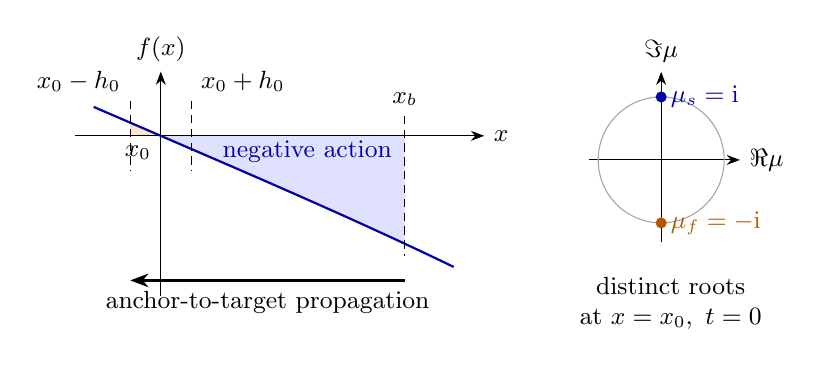
\begin{tikzpicture}[x=1.55cm,y=1.7cm,>=Stealth,font=\small]
 \def\del{0.03125}
 \fill[orange!20]plot[domain=-.25:0,samples=30]
  (\x,{2*ln(cot(180*(.25+\del*\x)))})--(0,0)--(-.25,0)--cycle;
 \fill[blue!12]plot[domain=0:2,samples=40]
  (\x,{2*ln(cot(180*(.25+\del*\x)))})--(2,0)--(0,0)--cycle;
 \draw[->](-.7,0)--(2.65,0)node[right]{$x$};
 \draw[->](0,-1.2)--(0,.48)node[above]{$f(x)$};
 \draw[thick,blue!65!black]plot[domain=-.55:2.4,samples=80]
  (\x,{2*ln(cot(180*(.25+\del*\x)))});
 \draw[densely dashed](-.25,.26)--(-.25,-.26);
 \draw[densely dashed](.25,.26)--(.25,-.26);
 \draw[densely dashed](2,.15)--(2,-.9);
 \node[above left]at(-.25,.26){$x_0-h_0$};
 \node[above right]at(.25,.26){$x_0+h_0$};
 \node[above]at(2,.15){$x_b$};
 \node[below left]at(0,0){$x_0$};
 \node[blue!65!black]at(1.2,-.12){negative action};
 \draw[<-,thick](-.25,-1.08)--(2,-1.08)
   node[midway,below]{anchor-to-target propagation};
 \begin{scope}[shift={(4.1,-.18)},x=.8cm,y=.8cm]
   \draw[->](-1.15,0)--(1.25,0)node[right]{$\Re\mu$};
   \draw[->](0,-1.3)--(0,1.4)node[above]{$\Im\mu$};
   \draw[black!35](0,0)circle(1);
   \fill[blue!65!black](0,1)circle(2pt)
     node[right]{$\mu_s=\ii$};
   \fill[orange!70!black](0,-1)circle(2pt)
     node[right]{$\mu_f=-\ii$};
   \node[below,align=center]at(.15,-1.7){distinct roots\\at $x=x_0,\ t=0$};
 \end{scope}
\end{tikzpicture}

 \caption{The relative logarithmic modulus $f(x)=2\log\cot(\pi x)$ changes sign at $x_0=1/4$. Both roots are nonzero and distinct there. The short positive area below quarter is outweighed by the negative area up to the fixed anchor $x_b$ for every target in $[x_0-\delta/4,x_0+\delta/4]$. The proof additionally bounds the absolute action accumulated to every intermediate index, so a conversion at such an index is controlled. Horizontal distances in the drawing are rescaled; the fixed width is chosen only after the analytic remainder barrier.}\label{qi:action-figure}
\end{figure}

\subsection{Both initial components come from the finite sum}

Shrink $t_0$ further to lie in the color disk of the high-index result on a fixed interval containing the anchor and its next index. This preserves all preceding action inequalities. At $x_b$ the high-index result of \cite[Section 3.2--3.3]{Conway} applies on a fixed compact interval above quarter and uniformly for complex $|t|<t_0$. Set
\[
 X_r=(U_{Nt,r},U_{Nt,r+1})^{\mathsf T},\qquad
 \begin{pmatrix}a_{s,N}(t)\\a_{f,N}(t)\end{pmatrix}
       =V_N(x_b,t)^{-1}X_{b_N}.
\]
These are exact entries defined from \eqref{qi:source}. The high-index theorem and $V_N=V_0+O(N^{-1})$ give
\begin{equation}\label{qi:anchor}
 a_{s,N}(t)=
 \frac{C(x_b,t)}{\mu_s(x_b,t)}
       e^{NS(x_b,t)}(1+O(N^{-1})),\qquad
 |a_{f,N}/a_{s,N}|\le C/N.
\end{equation}
To check the projection, the high-index ratio is
$U_{Nt,b_N}/U_{Nt,b_N+1}=\mu_s(x_b,t)+O(N^{-1})$.
Therefore $X_{b_N}$ is
$U_{Nt,b_N}\mu_s(x_b,t)^{-1}(\mu_s(x_b,t),1)^{\mathsf T}$
plus a relative $O(N^{-1})$ vector. Applying $V_N^{-1}$ gives
\eqref{qi:anchor}. In particular $a_{s,N}$ is holomorphic and nonzero on the fixed smaller disk. No conclusion about source overlap was drawn from the eigenvalues alone, and the second component is not set to zero.

By \eqref{qi:interaction} and \eqref{qi:partial-ratio},
\[
 \|E_j\|\le C e^{-3\sigma N/4},\qquad
 G_r^{-1}Y_r=
 \left[I+O(Ne^{-3\sigma N/4})\right]
       \begin{pmatrix}a_{s,N}\\a_{f,N}\end{pmatrix}.
\]
Let $v_1(x,t)=[V_N(x,t)]_{1,s}$. The first component after restoring $V_NG_r$ is therefore
\begin{equation}\label{qi:selected-source}
 U_{Nt,r}=a_{s,N}(t)v_1(r/N,t)G_s(r)
                 (1+O(e^{-c_1N}))
\end{equation}
for target indices and some $c_1>0$.
Indeed the direct fast term has relative size at most
$C N^{-1}e^{-6\pi\delta^2N}$ by \eqref{qi:anchor} and \eqref{qi:target-ratio}. The interaction error was bounded with the full partial-action width; at the target its fast output is smaller again. Bounded endpoint frames and their nonzero selected first component preserve these estimates. This proves a relative assertion for the original finite source with both channels retained.

\subsection{A fixed complex interpolation of the selected product}

Let $l_N(x,t)=\Log d_s(x,t)$, continuing $\Log\mu_s$. On a smaller fixed tube these logarithms are uniformly bounded and satisfy
$|\partial_x^j l_N|\le B j! a^{-j}$. Put $K_N=\lfloor c_2N\rfloor$, with $c_2>0$ sufficiently small, and define
\begin{align}
 E_N^s(x,t)={}&N\int_x^{x_b}l_N(u,t)\dd u
       +\frac{l_N(x,t)-l_N(x_b,t)}2\notag\\
 &+\sum_{k=1}^{K_N}\frac{B_{2k}N^{1-2k}}{(2k)!}
 \{\partial_x^{2k-1}l_N(x_b,t)
                 -\partial_x^{2k-1}l_N(x,t)\}.
 \label{qi:EM}
\end{align}
Here the Bernoulli numbers use $z/(e^z-1)=\sum B_jz^j/j!$.
The Euler--Maclaurin formula with periodic Bernoulli remainder
\cite[equation (2.10.1)]{DLMF}, applied separately to real and imaginary parts, gives the remainder for the actual product from $r$ to $b_N-1$. The Fourier series of the periodic Bernoulli polynomial
\cite[equation (24.8.1)]{DLMF} bounds its absolute value by
$4(2k)!/(2\pi)^{2k}$. Combining this with the Cauchy derivative estimate bounds the remainder by
\[
 CN\left(\frac{K_N}{\pi aN}\right)^{2K_N}\le C'e^{-c_3N};
\]
this follows from the displayed Cauchy bound and
$|B_{2k}|\le4(2k)!/(2\pi)^{2k}$.
It holds uniformly for the physical index grid and complex colors. Hence the explicit function
\begin{equation}\label{qi:I}
 I_N(x,t)=a_{s,N}(t)v_1(x,t)e^{E_N^s(x,t)}
\end{equation}
is holomorphic and nonzero on a fixed smaller joint domain, and
\eqref{qi:selected-source} proves \eqref{qi:grid}.
The anchor is an explicitly specified finite coefficient, not an unknown closed invariant. There is no interpolation of a moving support cutoff.

\subsection{Recovering the same leading amplitude}

It remains to show that \eqref{qi:I} has the leading expression in
\eqref{qi:complex}, including its normalization. The selected diagonal column of \eqref{qi:diagonal-identity} obeys the actual scalar recurrence up to an exponentially small relative defect. Its one-step scalar ratio is
\[
 v_{s,N}(x,t)=d_s(x,t)\frac{v_1(x,t)}{v_1(x+e,t)}.
\]
Both rows of the exact matrix identity imply
\begin{equation}\label{qi:Riccati}
 v_{s,N}(x,t)
 =p(x,t,e)+\frac{q_c(x,t,e)}{v_{s,N}(x+e,t)}
                        +O(e^{-\sigma' N})
\end{equation}
on a fixed smaller tube, for some $\sigma'>0$.
For example the second row gives
$v_1(x+e)=d_s(x)[V_N(x)]_{2,s}+O(e^{-\sigma N})$;
substitution in the first row, at $x$ and $x+e$, gives
\eqref{qi:Riccati}. All divisions use uniformly nonzero factors.

We know $v_{s,N}=\mu_s+O(e)$ with derivative bounds, but have not assumed a formal power series for it. Write $v_{s,N}=\mu_s+w_N$.
Cauchy's estimate gives $w_N'=O(e)$, so expanding
\eqref{qi:Riccati} yields
\[
 (1+q_0/\mu_s^2)w_N
 =e\{p_1+q_1/\mu_s-q_0\mu_{s,x}/\mu_s^2\}+O(e^2).
\]
The coefficient is $1-\mu_f/\mu_s$, uniformly separated from zero and equal to $2$ at quarter and $t=0$. Consequently
\begin{equation}\label{qi:first-correction}
 v_{s,N}=\mu_s+e\nu+O(e^2).
\end{equation}
Since $v_1=\mu_s+O(e)$ and $v_1'=\mu_s'+O(e)$, this implies
\[
 d_s=\mu_s+e(\nu+\mu_s')+O(e^2).
\]
Insert this expansion directly into \eqref{qi:EM}. Its higher Bernoulli terms have total size $O(N^{-1})$ on the smaller complex tube, by the same factorial estimates used for the exponential remainder. The extra integral of $\mu_s'/\mu_s$ equals
$\Log\mu_s(x_b)-\Log\mu_s(x)$. Combining it with the half-endpoint term and $v_1(x)/v_1(x_b)$ gives
\begin{align}
 \frac{v_1(x,t)e^{E_N^s(x,t)}}{v_1(x_b,t)}
 ={}&\sqrt{\frac{\mu_s(x,t)}{\mu_s(x_b,t)}}\notag\\
 &\times\exp\left\{
 N\int_x^{x_b}\Log\mu_s\,\dd u
       +\int_x^{x_b}\frac{\nu}{\mu_s}\,\dd u\right\}
       (1+O(N^{-1})).\label{qi:selected-leading}
\end{align}
This calculation holds at complex $x$; it is not a uniqueness argument on a finite mesh. At the anchor,
$a_{s,N}v_1(x_b)=C(x_b,t)e^{NS(x_b,t)}(1+O(N^{-1}))$
by \eqref{qi:anchor}. Multiplication in \eqref{qi:selected-leading} proves
\eqref{qi:complex} with exactly the $C,S$ of \eqref{qi:SC}.
Normalized remainders are holomorphic and uniformly bounded, so Cauchy's formula supplies the derivative statement. This completes the proof of Theorem~\ref{qi:main}.

At $t=0$ the values inherited from the original high-index normalization are, on both sides of quarter,
\[
 S(x,0)=\pi\ii(1/2-x)^2,\qquad
 C(x,0)=\sqrt{\sin\pi x}\,e^{-3\pi\ii(1/2-x)/2}.
\]
No connection constant or parity-dependent factor has been chosen at the crossing.

\section{Signed leaves and strict finite wire windows}\label{qi:signed}

The preceding theorem was stated for a normalized scalar recurrence. We now restore its actual tangle coefficient. Let
$S_r=\prod_{a=1}^r2\sin(\pi a/N)$.
For an integer wire $r$ near quarter and $h=Nt$, the original pure coefficient and its retained half twist are
\begin{align}
 A_N(r,t)&=\frac{N^2S_{2r}}
 {S_r^2G_N(r-Nt)G_N(r+Nt)},\notag\\
 d_N^\epsilon(r,t)&=\kappa^\epsilon
 \sum_{v=r}^M(-1)^v q^{\epsilon v(r+1)}
                   \frac{S_v}{S_rS_{v-r}}A_N(v,t),
       \quad\epsilon=\pm1,\qquad d_N^0=A_N.\label{qi:signed-source}
\end{align}
The sign $\epsilon$ denotes a physical retained crossing and is distinct from the step $e=1/N$. Put
$\ell_N^\epsilon=e^{-\pi\ii\epsilon d/4}d_N^\epsilon$.

\begin{corollary}[The signed coefficient and its absolute action]\label{qi:signed-corollary}
The coefficients $\ell_N^\epsilon$ admit nonzero holomorphic interpolants
$I_N^\epsilon(x,t)$ on a fixed joint neighborhood of $(1/4,0)$ with
\[
 \ell_N^\epsilon(r,t)=I_N^\epsilon(r/N,t)
                     (1+O(e^{-cN})),\qquad
 I_N^\epsilon=N^{1/2}b_\epsilon e^{Nf_\epsilon}
                     (1+O(N^{-1})).
\]
The first assertion is on the physical index grid and the second on a fixed complex domain. The amplitudes are nonzero, the functions are even in $t$, and
\begin{align}
 g(x,t)&=J(2x)-2J(x)-J(x-t)-J(x+t),\notag\\
 f_0&=g,\qquad f_-=g+S(x,t)-S(x,0),\qquad
 f_+(x,t)=\overline{f_-(\bar x,\bar t)}.\label{qi:actions}
\end{align}
Here $J'(z)=\Log(2\sin\pi z)$ is normalized by $J(0)=0$.
Equivalently, the small solution of
\begin{equation}\label{qi:shear}
 t=s-\frac{\epsilon g_s(x,s)}{2\pi\ii}
\end{equation}
satisfies the exact identity
\begin{equation}\label{qi:absolute-shear}
 f_\epsilon(x,t)=g(x,s)
                   -\frac{\epsilon g_s(x,s)^2}{4\pi\ii}.
\end{equation}
In particular
\[
 \frac{b_\epsilon(x,0)}{b_0(x,0)}
   =\sqrt{\sin\pi x}\,e^{-\epsilon\pi\ii x/2}
       \quad(\epsilon=\pm1),\qquad
 (f_\epsilon)_{tt}(x,0)
       =-\frac{2\pi\cot(\pi x)}{1-\epsilon\ii\cot(\pi x)}.
\]
\end{corollary}

\begin{proof}
Define
\begin{align}
 A_N^{\rm hol}(x,t)
 &=\frac{N^2G_N(2Nx)}
        {G_N(Nx)^2G_N(N(x-t))G_N(N(x+t))},\notag\\
 P_N^{\rm ch}(x)
 &=\frac{\kappa^{-1}e^{\pi\ii d/4}}
        {e^{-\pi\ii Nx+\pi\ii Nx(Nx+1)/N}},\notag\\
 I_N^-&=A_N^{\rm hol}P_N^{\rm ch}I_N,\qquad
 I_N^+(x,t)=\overline{I_N^-(\bar x,\bar t)},\qquad
 I_N^0=A_N^{\rm hol}.\label{qi:actual-interpolants}
\end{align}
The finite algebra connecting \eqref{qi:source} and
\eqref{qi:signed-source} is unchanged at quarter. Explicitly,
\[
 q^{h^2}\frac{D_{h,r}}{D_{0,r}}
   =\frac{G_N(r)^2}{G_N(r-h)G_N(r+h)}.
\]
The chirp $q^{h^2}$ is therefore retained in
\eqref{qi:actual-interpolants}. Substitution gives the claimed exponentially accurate grid identity by Theorem~\ref{qi:main}. All factorial arguments now lie on fixed regular compact substrips, so the canonical bulk expansion \cite[Lemma 2.1]{Conway} applies. It gives \eqref{qi:actions} and the explicit nonzero densities
\begin{align}
 b_0(x,t)&=
 \frac{\sqrt{\sin2\pi x}}
 {2^{3/2}\sin\pi x\sqrt{\sin\pi(x-t)\sin\pi(x+t)}},\notag\\
 b_-(x,t)&=b_0(x,t)e^{\pi\ii(3/4-x)}C(x,t),\qquad
 b_+(x,t)=\overline{b_-(\bar x,\bar t)}.\label{qi:density}
\end{align}
All marks continue those fixed at the upper endpoint; no new square-root choice is made here.

For $x$ above quarter the absolute identity
\eqref{qi:absolute-shear} is \cite[Proposition 3.1]{Conway}, including its additive function of color. Both sides extend holomorphically to the connected neighborhood just constructed. The derivative of \eqref{qi:shear} in $s$ at zero is
$1-\epsilon\ii\cot(\pi x)$, which stays nonzero there. The identity theorem therefore extends the already normalized equality through quarter. It is not an inference from the second derivative alone.
Formula \eqref{qi:density} and the complete $C$ at the end of Section~\ref{qi:source-proof} give the amplitude ratio. Differentiating the exact shear gives the displayed color Hessian.
\end{proof}

\subsection{An application with explicit local hypotheses}

The following consequence concerns an exact finite window in an original Newton contraction. It has no assumption about the contribution outside that window.

\begin{corollary}[A local finite-window Gaussian]\label{qi:window}
Fix a finite Newton contraction with $b$ leaf factors
\eqref{qi:signed-source}, $g$ retained multiplication gates, and $k$ free primitive integer wire coordinates. Suppose a strict real state $y_0$ has the following properties:
\begin{enumerate}
 \item Every wire has its actual form $r_w=NL_w(y)+\delta_w$, with $L_w$ integral affine and $\delta_w$ a fixed integer. The retained summation lattice is all of $\mathbb Z^k$ in these coordinates.
 \item All factorial arguments of every retained gate are strictly between $0$ and $N$ at the limiting state, and every leaf coordinate lies in the union of the quarter neighborhood of Theorem~\ref{qi:main} and fixed compact intervals in $(1/4,1/2)$.
 \item The pure limiting phase is stationary at $y_0$ and has negative definite Hessian there.
\end{enumerate}
Choose a sufficiently small fixed rectangular window about $y_0$, and let $C_N^\epsilon(t)$ be its exact finite sum with the normalized leaves $\ell_N^\epsilon$ and the original integer gate coefficients. There are nonzero holomorphic $a_\epsilon(t)$ and even holomorphic $\Phi_\epsilon(t)$ on a fixed polydisk such that
\begin{equation}\label{qi:window-asymptotic}
 C_N^\epsilon(t)=
 N^{b/2-3g/2+k/2}a_\epsilon(t)e^{N\Phi_\epsilon(t)}
                         (1+O(N^{-1}))
\end{equation}
uniformly there, with both level parities retained. For a binary cylindrical closure with one eliminated closing equation, $g=b-2$ and $k=2b-3$, so the power is $3/2$. The original unnormalized window has the additional factor
$e^{\pi\ii d\sum\epsilon_\ell/4}$.
Its diagonal color Hessian is
\[
 (\Phi_\epsilon)_{t_\ell t_j}(0)=
 -\frac{2\pi\cot(\pi a_\ell)}
       {1-\epsilon_\ell\ii\cot(\pi a_\ell)}\,
       \mathbf1_{\ell=j},
 \qquad a_\ell=L_\ell(y_0).
\]
\end{corollary}

\begin{proof}
The multiplication formula of \cite[Theorem 3.3]{Newton} is
\[
 \mu_N(i,j,r)=
 \frac{S_{i+j}S_r}{S_iS_jS_{r-i}S_{r-j}S_{i+j-r}},
 \qquad \max(i,j)\le r\le i+j\le d .
\]
In a strict window its canonical interpolation has power $N^{-3/2}$,
nonzero leading density, and phase
\[
 m(x,y,z)=J(x+y)+J(z)-J(x)-J(y)
                  -J(z-x)-J(z-y)-J(x+y-z).
\]
Together with Corollary~\ref{qi:signed-corollary} and the high-index theorem this gives an interpolated summand
\[
 N^{b/2-3g/2}b_\epsilon(y,t)e^{NF_\epsilon(y,t)}
                         (1+O(N^{-1})).
\]
Here $F_\epsilon$ is the sum of the actual leaf actions and gate actions. The density multiplies the leaf and gate densities and every offset factor:
$e^{\delta_\ell\partial_xf_{\epsilon_\ell}}$ for a leaf and
$e^{\delta_i m_x+\delta_j m_y+\delta_r m_z}$ for a gate.
They are evaluated at the changed variables, not at the complete point. All are nonzero.

The difference from the exact finite summand is exponentially small relative to the product of absolute local factors. On the real complete window its total absolute sum is bounded by
$N^C e^{N(F_0-c)}$, where $F_0=F_\epsilon(y_0,0)$ and $c>0$ is smaller than the finite minimum of the interpolation exponents. For complex small colors the bound is
$N^C e^{N(F_0+C_1\|t\|^2-c)}$.
Shrinking the color disk keeps this error below the selected critical action. Thus the errors were estimated before the complex saddle, not appended after a potentially cancelling sum.

At zero the phase is independent of the retained signs and has the specified negative definite Hessian. The holomorphic implicit-function theorem supplies its unique nearby critical point $y_*(t)$. Put
\[
 \Phi_\epsilon(t)=F_\epsilon(y_*(t),t),\qquad
 a_\epsilon(t)=
 \frac{(2\pi)^{k/2}b_\epsilon(y_*(t),t)}
 {\sqrt{\det[-(F_\epsilon)_{yy}(y_*(t),t)]}}.
\]
To identify its coefficient in the finite sum, enclose each index interval by a rectangle with vertical half-grid sides and heights $\pm a$. The exact residue kernel $\pi N\cot(\pi Nz)$ has residue one at each retained $j/N$. Vertical sides keep the fixed real boundary loss. Horizontal sides have constant terms $\mp\ii$ and error $O(e^{-2\pi Na})$. Choose $a$ first so its $O(a^2)$ phase cost is less than one quarter of the real boundary gap and less than $\pi a$; then shrink the complex color disk. All boundary and nonconstant-kernel terms are exponentially smaller. Iterating gives $N^k$ times the ordinary integral over the rectangle with exponentially small error. Because the integer coordinates are primitive, there is no extra density factor.

Translate the integral to the parallel real contour through $y_*(t)$. Its connecting boundary faces retain the loss; the local negative Hessian has positive real part. Gaussian integration gives the coefficient and power in \eqref{qi:window-asymptotic}. Odd Taylor terms have zero Gaussian integral, so the relative error is $O(N^{-1})$, uniformly holomorphically. At zero the density differs from the positive pure density by
$\prod_{\epsilon_\ell\ne0}\sqrt{\sin\pi a_\ell}
 e^{-\epsilon_\ell\pi\ii a_\ell/2}$, which is nonzero.
Finally evenness makes all mixed wire--color derivatives vanish at zero, and the local color Hessian in Corollary~\ref{qi:signed-corollary} gives the displayed formula.
\end{proof}

\section{Reproduction and limits of the conclusion}\label{qi:checks}

The paper-local command
\[
 \texttt{python3 -I papers/quarter-index-asymptotics/check.py}
\]
uses Python's standard library and writes a JSON record to its paper-local build directory; \texttt{--output} selects another directory.
It checks the recurrence directly from the original finite factorial sum over finite fields at both parities, including its terminal zero. Independently chosen rational matrices test the exact backward conjugation formula and the two-channel interaction reconstruction, retaining both input components. Input hashes are recorded before and after the run and an earlier summary is removed before validation.

These are finite algebra checks of the direction, normalization and endpoint identities. They do not prove the analytic bounds or infer an all-level theorem from examples. The analytic proof chooses a fixed recurrence domain and its exponential barrier first, then the shorter crossing width, then the complex color disk, and only then lets $N$ grow. It controls a short regular modulus crossing. It does not continue the selected solution arbitrarily far below quarter, pass through colliding roots, discard a global alias, or evaluate an entire filled invariant. Any such application requires its own global source and geometric inputs.


\begin{thebibliography}{9}
\bibitem{Conway}\emph{Holomorphic source asymptotics and volume limits for Conway closures}.
Companion paper, \href{https://sashakolpakov.github.io/murakamis_dream/papers/conway-asymptotics.pdf}{repository edition}.
\bibitem{Newton}\emph{Newton coefficients and positive sources for Conway tangles}.
Companion paper, \href{https://sashakolpakov.github.io/murakamis_dream/papers/newton-tangles.pdf}{repository edition}.
\bibitem{CostinCostin} O. Costin and R. D. Costin,
\emph{Rigorous WKB for finite-order linear recurrence relations with smooth coefficients},
SIAM J. Math. Anal. \textbf{27} (1996), no.~1, 110--134;
\href{https://arxiv.org/abs/math/0608413}{author preprint}.
\bibitem{DLMF} F. W. J. Olver et al., eds.,
\emph{NIST Digital Library of Mathematical Functions},
\href{https://dlmf.nist.gov/2.10.E1}{equation (2.10.1)} and
\href{https://dlmf.nist.gov/24.8.E1}{equation (24.8.1)}.
\end{thebibliography}
\end{document}
